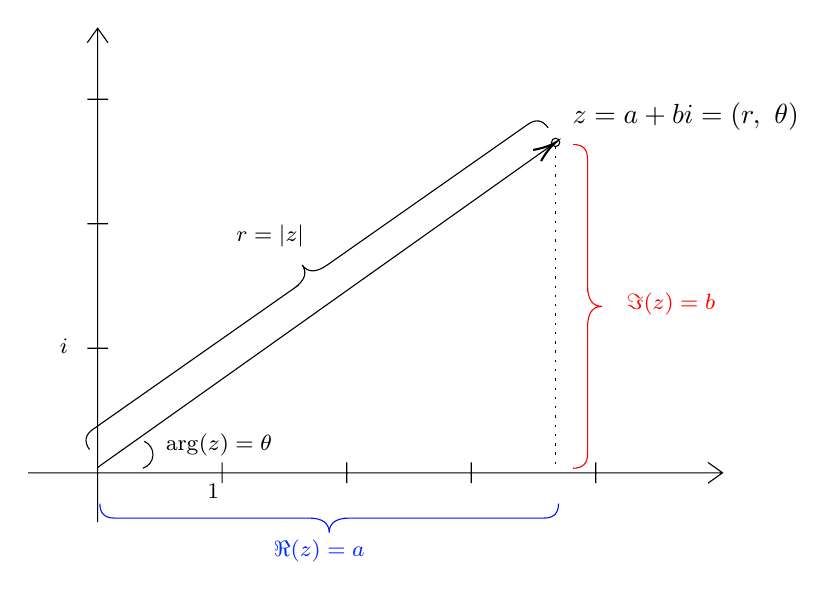
\begin{tikzpicture}[x=0.75pt,y=0.75pt,yscale=-1,xscale=1]
%uncomment if require: \path (0,300); %set diagram left start at 0, and has height of 300

%Shape: Axis 2D [id:dp4700217616893223] 
\draw  (46,246.2) -- (380.5,246.2)(79.45,32) -- (79.45,270) (373.5,241.2) -- (380.5,246.2) -- (373.5,251.2) (74.45,39) -- (79.45,32) -- (84.45,39) (139.45,241.2) -- (139.45,251.2)(199.45,241.2) -- (199.45,251.2)(259.45,241.2) -- (259.45,251.2)(319.45,241.2) -- (319.45,251.2)(74.45,186.2) -- (84.45,186.2)(74.45,126.2) -- (84.45,126.2)(74.45,66.2) -- (84.45,66.2) ;
\draw   ;
%Straight Lines [id:da1141401634967012] 
\draw    (79.45,243.6) -- (298.47,88.16) ;
\draw [shift={(300.1,87)}, rotate = 504.64] [color={rgb, 255:red, 0; green, 0; blue, 0 }  ][line width=0.75]    (10.93,-3.29) .. controls (6.95,-1.4) and (3.31,-0.3) .. (0,0) .. controls (3.31,0.3) and (6.95,1.4) .. (10.93,3.29)   ;
%Shape: Circle [id:dp44110533792950923] 
\draw   (298.1,87) .. controls (298.1,85.9) and (299,85) .. (300.1,85) .. controls (301.2,85) and (302.1,85.9) .. (302.1,87) .. controls (302.1,88.1) and (301.2,89) .. (300.1,89) .. controls (299,89) and (298.1,88.1) .. (298.1,87) -- cycle ;
%Shape: Arc [id:dp03726885849887451] 
\draw  [draw opacity=0] (101.9,231.06) .. controls (104.44,232.14) and (106.18,234.69) .. (106.1,237.61) .. controls (106.01,240.63) and (103.98,243.14) .. (101.25,243.99) -- (99.21,237.4) -- cycle ; \draw   (101.9,231.06) .. controls (104.44,232.14) and (106.18,234.69) .. (106.1,237.61) .. controls (106.01,240.63) and (103.98,243.14) .. (101.25,243.99) ;
%Shape: Brace [id:dp38892828645713595] 
\draw   (296.5,80) .. controls (293.82,76.18) and (290.57,75.61) .. (286.75,78.29) -- (190.16,146.02) .. controls (184.71,149.85) and (180.64,149.85) .. (177.96,146.03) .. controls (180.64,149.85) and (179.25,153.67) .. (173.79,157.5)(176.24,155.78) -- (77.2,225.23) .. controls (73.38,227.91) and (72.81,231.16) .. (75.49,234.98) ;
%Shape: Brace [id:dp00822474139118512] 
\draw  [color={rgb, 255:red, 0; green, 15; blue, 255 }  ,draw opacity=1 ] (80.5,261) .. controls (80.5,265.67) and (82.83,268) .. (87.5,268) -- (181,268) .. controls (187.67,268) and (191,270.33) .. (191,275) .. controls (191,270.33) and (194.33,268) .. (201,268)(198,268) -- (294.5,268) .. controls (299.17,268) and (301.5,265.67) .. (301.5,261) ;
%Shape: Brace [id:dp4128906105867539] 
\draw  [color={rgb, 255:red, 255; green, 0; blue, 0 }  ,draw opacity=1 ] (308.5,244) .. controls (313.17,244) and (315.5,241.67) .. (315.5,237) -- (315.5,176) .. controls (315.5,169.33) and (317.83,166) .. (322.5,166) .. controls (317.83,166) and (315.5,162.67) .. (315.5,156)(315.5,159) -- (315.5,95) .. controls (315.5,90.33) and (313.17,88) .. (308.5,88) ;
%Straight Lines [id:da26429163876661155] 
\draw  [dash pattern={on 0.84pt off 2.51pt}]  (300.1,89) -- (300.1,245) ;

% Text Node
\draw (60,180.4) node [anchor=north west][inner sep=0.75pt]  [font=\footnotesize]  {$i$};
% Text Node
\draw (131,250.4) node [anchor=north west][inner sep=0.75pt]  [font=\footnotesize]  {$1$};
% Text Node
\draw (111,226.4) node [anchor=north west][inner sep=0.75pt]  [font=\footnotesize]  {$\arg( z) =\theta $};
% Text Node
\draw (333,158.4) node [anchor=north west][inner sep=0.75pt]  [font=\footnotesize,color={rgb, 255:red, 255; green, 0; blue, 0 }  ,opacity=1 ]  {$\Im ( z) =b$};
% Text Node
\draw (163,277.4) node [anchor=north west][inner sep=0.75pt]  [font=\footnotesize,color={rgb, 255:red, 0; green, 42; blue, 255 }  ,opacity=1 ]  {$\Re ( z) =a$};
% Text Node
\draw (145,125.4) node [anchor=north west][inner sep=0.75pt]  [font=\footnotesize]  {$r=|z|$};
% Text Node
\draw (307,66.4) node [anchor=north west][inner sep=0.75pt]    {$z=a+bi=( r,\ \theta )$};


\end{tikzpicture}